
%% bare_conf.tex
%% V1.4b
%% 2015/08/26
%% by Michael Shell
%% See:
%% http://www.michaelshell.org/
%% for current contact information.
%%
%% This is a skeleton file demonstrating the use of IEEEtran.cls
%% (requires IEEEtran.cls version 1.8b or later) with an IEEE
%% conference paper.
%%
%% Support sites:
%% http://www.michaelshell.org/tex/ieeetran/
%% http://www.ctan.org/pkg/ieeetran
%% and
%% http://www.ieee.org/

%%*************************************************************************
%% Legal Notice:
%% This code is offered as-is without any warranty either expressed or
%% implied; without even the implied warranty of MERCHANTABILITY or
%% FITNESS FOR A PARTICULAR PURPOSE!
%% User assumes all risk.
%% In no event shall the IEEE or any contributor to this code be liable for
%% any damages or losses, including, but not limited to, incidental,
%% consequential, or any other damages, resulting from the use or misuse
%% of any information contained here.
%%
%% All comments are the opinions of their respective authors and are not
%% necessarily endorsed by the IEEE.
%%
%% This work is distributed under the LaTeX Project Public License (LPPL)
%% ( http://www.latex-project.org/ ) version 1.3, and may be freely used,
%% distributed and modified. A copy of the LPPL, version 1.3, is included
%% in the base LaTeX documentation of all distributions of LaTeX released
%% 2003/12/01 or later.
%% Retain all contribution notices and credits.
%% ** Modified files should be clearly indicated as such, including  **
%% ** renaming them and changing author support contact information. **
%%*************************************************************************


% *** Authors should verify (and, if needed, correct) their LaTeX system  ***
% *** with the testflow diagnostic prior to trusting their LaTeX platform ***
% *** with production work. The IEEE's font choices and paper sizes can   ***
% *** trigger bugs that do not appear when using other class files.       ***                          ***
% The testflow support page is at:
% http://www.michaelshell.org/tex/testflow/



\documentclass[conference]{IEEEtran}
% Some Computer Society conferences also require the compsoc mode option,
% but others use the standard conference format.
%
% If IEEEtran.cls has not been installed into the LaTeX system files,
% manually specify the path to it like:
% \documentclass[conference]{../sty/IEEEtran}





% Some very useful LaTeX packages include:
% (uncomment the ones you want to load)


% *** MISC UTILITY PACKAGES ***
%
%\usepackage{ifpdf}
% Heiko Oberdiek's ifpdf.sty is very useful if you need conditional
% compilation based on whether the output is pdf or dvi.
% usage:
% \ifpdf
%   % pdf code
% \else
%   % dvi code
% \fi
% The latest version of ifpdf.sty can be obtained from:
% http://www.ctan.org/pkg/ifpdf
% Also, note that IEEEtran.cls V1.7 and later provides a builtin
% \ifCLASSINFOpdf conditional that works the same way.
% When switching from latex to pdflatex and vice-versa, the compiler may
% have to be run twice to clear warning/error messages.






% *** CITATION PACKAGES ***
%
\usepackage{cite}
\usepackage[hidelinks]{hyperref}
\usepackage{supertabular,amssymb}
% cite.sty was written by Donald Arseneau
% V1.6 and later of IEEEtran pre-defines the format of the cite.sty package
% \cite{} output to follow that of the IEEE. Loading the cite package will
% result in citation numbers being automatically sorted and properly
% "compressed/ranged". e.g., [1], [9], [2], [7], [5], [6] without using
% cite.sty will become [1], [2], [5]--[7], [9] using cite.sty. cite.sty's
% \cite will automatically add leading space, if needed. Use cite.sty's
% noadjust option (cite.sty V3.8 and later) if you want to turn this off
% such as if a citation ever needs to be enclosed in parenthesis.
% cite.sty is already installed on most LaTeX systems. Be sure and use
% version 5.0 (2009-03-20) and later if using hyperref.sty.
% The latest version can be obtained at:
% http://www.ctan.org/pkg/cite
% The documentation is contained in the cite.sty file itself.






% *** GRAPHICS RELATED PACKAGES ***
%
\ifCLASSINFOpdf
  % \usepackage[pdftex]{graphicx}
  % declare the path(s) where your graphic files are
  % \graphicspath{{../pdf/}{../jpeg/}}
  % and their extensions so you won't have to specify these with
  % every instance of \includegraphics
  % \DeclareGraphicsExtensions{.pdf,.jpeg,.png}
\else
  % or other class option (dvipsone, dvipdf, if not using dvips). graphicx
  % will default to the driver specified in the system graphics.cfg if no
  % driver is specified.
  % \usepackage[dvips]{graphicx}
  % declare the path(s) where your graphic files are
  % \graphicspath{{../eps/}}
  % and their extensions so you won't have to specify these with
  % every instance of \includegraphics
  % \DeclareGraphicsExtensions{.eps}
\fi
% graphicx was written by David Carlisle and Sebastian Rahtz. It is
% required if you want graphics, photos, etc. graphicx.sty is already
% installed on most LaTeX systems. The latest version and documentation
% can be obtained at:
% http://www.ctan.org/pkg/graphicx
% Another good source of documentation is "Using Imported Graphics in
% LaTeX2e" by Keith Reckdahl which can be found at:
% http://www.ctan.org/pkg/epslatex
%
% latex, and pdflatex in dvi mode, support graphics in encapsulated
% postscript (.eps) format. pdflatex in pdf mode supports graphics
% in .pdf, .jpeg, .png and .mps (metapost) formats. Users should ensure
% that all non-photo figures use a vector format (.eps, .pdf, .mps) and
% not a bitmapped formats (.jpeg, .png). The IEEE frowns on bitmapped formats
% which can result in "jaggedy"/blurry rendering of lines and letters as
% well as large increases in file sizes.
%
% You can find documentation about the pdfTeX application at:
% http://www.tug.org/applications/pdftex
\usepackage{graphicx}
\usepackage{caption}
\usepackage{subcaption}
\usepackage{wrapfig}




% *** MATH PACKAGES ***
%
\usepackage{amsmath}
% A popular package from the American Mathematical Society that provides
% many useful and powerful commands for dealing with mathematics.
%
% Note that the amsmath package sets \interdisplaylinepenalty to 10000
% thus preventing page breaks from occurring within multiline equations. Use:
%\interdisplaylinepenalty=2500
% after loading amsmath to restore such page breaks as IEEEtran.cls normally
% does. amsmath.sty is already installed on most LaTeX systems. The latest
% version and documentation can be obtained at:
% http://www.ctan.org/pkg/amsmath





% *** SPECIALIZED LIST PACKAGES ***
%
\usepackage{algorithmic}
% algorithmic.sty was written by Peter Williams and Rogerio Brito.
% This package provides an algorithmic environment fo describing algorithms.
% You can use the algorithmic environment in-text or within a figure
% environment to provide for a floating algorithm. Do NOT use the algorithm
% floating environment provided by algorithm.sty (by the same authors) or
% algorithm2e.sty (by Christophe Fiorio) as the IEEE does not use dedicated
% algorithm float types and packages that provide these will not provide
% correct IEEE style captions. The latest version and documentation of
% algorithmic.sty can be obtained at:
% http://www.ctan.org/pkg/algorithms
% Also of interest may be the (relatively newer and more customizable)
% algorithmicx.sty package by Szasz Janos:
% http://www.ctan.org/pkg/algorithmicx




% *** ALIGNMENT PACKAGES ***
%
%\usepackage{array}
% Frank Mittelbach's and David Carlisle's array.sty patches and improves
% the standard LaTeX2e array and tabular environments to provide better
% appearance and additional user controls. As the default LaTeX2e table
% generation code is lacking to the point of almost being broken with
% respect to the quality of the end results, all users are strongly
% advised to use an enhanced (at the very least that provided by array.sty)
% set of table tools. array.sty is already installed on most systems. The
% latest version and documentation can be obtained at:
% http://www.ctan.org/pkg/array


% IEEEtran contains the IEEEeqnarray family of commands that can be used to
% generate multiline equations as well as matrices, tables, etc., of high
% quality.




% *** SUBFIGURE PACKAGES ***
%\ifCLASSOPTIONcompsoc
%  \usepackage[caption=false,font=normalsize,labelfont=sf,textfont=sf]{subfig}
%\else
%  \usepackage[caption=false,font=footnotesize]{subfig}
%\fi
% subfig.sty, written by Steven Douglas Cochran, is the modern replacement
% for subfigure.sty, the latter of which is no longer maintained and is
% incompatible with some LaTeX packages including fixltx2e. However,
% subfig.sty requires and automatically loads Axel Sommerfeldt's caption.sty
% which will override IEEEtran.cls' handling of captions and this will result
% in non-IEEE style figure/table captions. To prevent this problem, be sure
% and invoke subfig.sty's "caption=false" package option (available since
% subfig.sty version 1.3, 2005/06/28) as this is will preserve IEEEtran.cls
% handling of captions.
% Note that the Computer Society format requires a larger sans serif font
% than the serif footnote size font used in traditional IEEE formatting
% and thus the need to invoke different subfig.sty package options depending
% on whether compsoc mode has been enabled.
%
% The latest version and documentation of subfig.sty can be obtained at:
% http://www.ctan.org/pkg/subfig




% *** FLOAT PACKAGES ***
%
%\usepackage{fixltx2e}
% fixltx2e, the successor to the earlier fix2col.sty, was written by
% Frank Mittelbach and David Carlisle. This package corrects a few problems
% in the LaTeX2e kernel, the most notable of which is that in current
% LaTeX2e releases, the ordering of single and double column floats is not
% guaranteed to be preserved. Thus, an unpatched LaTeX2e can allow a
% single column figure to be placed prior to an earlier double column
% figure.
% Be aware that LaTeX2e kernels dated 2015 and later have fixltx2e.sty's
% corrections already built into the system in which case a warning will
% be issued if an attempt is made to load fixltx2e.sty as it is no longer
% needed.
% The latest version and documentation can be found at:
% http://www.ctan.org/pkg/fixltx2e


%\usepackage{stfloats}
% stfloats.sty was written by Sigitas Tolusis. This package gives LaTeX2e
% the ability to do double column floats at the bottom of the page as well
% as the top. (e.g., "\begin{figure*}[!b]" is not normally possible in
% LaTeX2e). It also provides a command:
%\fnbelowfloat
% to enable the placement of footnotes below bottom floats (the standard
% LaTeX2e kernel puts them above bottom floats). This is an invasive package
% which rewrites many portions of the LaTeX2e float routines. It may not work
% with other packages that modify the LaTeX2e float routines. The latest
% version and documentation can be obtained at:
% http://www.ctan.org/pkg/stfloats
% Do not use the stfloats baselinefloat ability as the IEEE does not allow
% \baselineskip to stretch. Authors submitting work to the IEEE should note
% that the IEEE rarely uses double column equations and that authors should try
% to avoid such use. Do not be tempted to use the cuted.sty or midfloat.sty
% packages (also by Sigitas Tolusis) as the IEEE does not format its papers in
% such ways.
% Do not attempt to use stfloats with fixltx2e as they are incompatible.
% Instead, use Morten Hogholm'a dblfloatfix which combines the features
% of both fixltx2e and stfloats:
%
% \usepackage{dblfloatfix}
% The latest version can be found at:
% http://www.ctan.org/pkg/dblfloatfix




% *** PDF, URL AND HYPERLINK PACKAGES ***
%
%\usepackage{url}
% url.sty was written by Donald Arseneau. It provides better support for
% handling and breaking URLs. url.sty is already installed on most LaTeX
% systems. The latest version and documentation can be obtained at:
% http://www.ctan.org/pkg/url
% Basically, \url{my_url_here}.




% *** Do not adjust lengths that control margins, column widths, etc. ***
% *** Do not use packages that alter fonts (such as pslatex).         ***
% There should be no need to do such things with IEEEtran.cls V1.6 and later.
% (Unless specifically asked to do so by the journal or conference you plan
% to submit to, of course. )


% correct bad hyphenation here
\hyphenation{op-tical net-works semi-conduc-tor}


\begin{document}
%
% paper title
% Titles are generally capitalized except for words such as a, an, and, as,
% at, but, by, for, in, nor, of, on, or, the, to and up, which are usually
% not capitalized unless they are the first or last word of the title.
% Linebreaks \\ can be used within to get better formatting as desired.
% Do not put math or special symbols in the title.
\title{Measuring Hash Trustworthiness via Collision Utility Metrics: Logical Cryptanalysis of MD4}


% author names and affiliations
% use a multiple column layout for up to three different
% affiliations
\author{\IEEEauthorblockN{Alexander M. Scheel, Eric W. D. Rozier}
\IEEEauthorblockA{Department of Computer Science\\Iowa State University of Science and Technology\\
Ames, Iowa, USA 50011\\
Email: \texttt{alexander.m.scheel@gmail.com, erozier@iastate.edu}}}
% conference papers do not typically use \thanks and this command
% is locked out in conference mode. If really needed, such as for
% the acknowledgment of grants, issue a \IEEEoverridecommandlockouts
% after \documentclass

% for over three affiliations, or if they all won't fit within the width
% of the page, use this alternative format:
%
%\author{\IEEEauthorblockN{Michael Shell\IEEEauthorrefmark{1},
%Homer Simpson\IEEEauthorrefmark{2},
%James Kirk\IEEEauthorrefmark{3},
%Montgomery Scott\IEEEauthorrefmark{3} and
%Eldon Tyrell\IEEEauthorrefmark{4}}
%\IEEEauthorblockA{\IEEEauthorrefmark{1}School of Electrical and Computer Engineering\\
%Georgia Institute of Technology,
%Atlanta, Georgia 30332--0250\\ Email: see http://www.michaelshell.org/contact.html}
%\IEEEauthorblockA{\IEEEauthorrefmark{2}Twentieth Century Fox, Springfield, USA\\
%Email: homer@thesimpsons.com}
%\IEEEauthorblockA{\IEEEauthorrefmark{3}Starfleet Academy, San Francisco, California 96678-2391\\
%Telephone: (800) 555--1212, Fax: (888) 555--1212}
%\IEEEauthorblockA{\IEEEauthorrefmark{4}Tyrell Inc., 123 Replicant Street, Los Angeles, California 90210--4321}}




% use for special paper notices
%\IEEEspecialpapernotice{(Invited Paper)}




% make the title area
\maketitle

% As a general rule, do not put math, special symbols or citations
% in the abstract
\begin{abstract}
The discovery of fast collision attacks in cryptographic hash functions has
traditionally resulted in the immediate deprecation of that hash function.
In this paper we propose five scalable and practical metrics for evaluating
the utility of collision classes based on boolean constraints and show that
the published attacks by X. Wang, Y. Sasaki, P. Kasselman, H. Dobbertin, and
M. Schl{\"a}ffer in MD4 have high utility. We expand on existing attacks by
developing a series of techniques based on logical cryptanalysis to find
over 35,000 collisions in MD4 based on existing collisions, through the novel
definition of a collision neighborhood. We demonstrate new techniques for
inductively building full collisions from reduced round variants of MD4. We
propose these techniques as a mechanism for measuring hash trustworthiness and
discuss potential applications to real-world systems.
\end{abstract}

% no keywords
% For peer review papers, you can put extra information on the cover
% page as needed:
% \ifCLASSOPTIONpeerreview
% \begin{center} \bfseries EDICS Category: 3-BBND \end{center}
% \fi
%
% For peerreview papers, this IEEEtran command inserts a page break and
% creates the second title. It will be ignored for other modes.
\IEEEpeerreviewmaketitle

\section{Introduction}

Cryptographic hash functions form the core of many protocols which
trust that cryptographic hash functions preserve certain basic
properties. Cryptograpic hash functions see widespread
use for file integrity checks to verify long term storage of
data, as cache invalidation techniques, and as a building block in network
protocols such as Kerberos and TLS.  The classes of functions suitable
for these use cases necessarily have
strong guarantees about properties of its members. 
An ideal cryptographic hash has five main features: determinism - the
same message always results in the same hash; performability -
computing a hash for a message should not be algorithmically
difficult; non-reversability - it should be infeasible to generate a message
from its hash except by trying all possible messages; sensitivity to
initial conditions - small changes to a message should change the hash
value to a degree that the new hash value appears uncorrelated with
the old hash value; unique digests - it should be infeasible to find
two different messages with the same hash value.

The most important aspect of these can be formally defined under three
properties which hash function implementations must have to be
considered cryptographically secure in practice:
\begin{itemize}
    \item \textbf{Preimage Resistance}: It should be computationally hard to find
        the inverse of a hash function.
    \item \textbf{Second Preimage Resistance}: Given an input block, it should be
        computationally hard to find a second block which hashes to the
        same value as the first block.
    \item \textbf{Collision Resistance}: It should be computationally hard to find two
        blocks which hash to the same value.
\end{itemize}
Note that while a second preimage is necessarily a collision, it is also a
stronger result with higher use for an attacker.

From an attacker's perspective, finding a preimage or second preimage has been
difficult: the current published bound for a preimage attack in MD5 is a cost
of $2^{123.4}$ by Y. Sasaki and K. Aoki \cite{SasakiPreimage}. In MD4, the
best second preimage attack by H. Yu et al. gives a bound of $\frac{1}{2^{56}}$
likelihood, but uses destructive message modification techniques to achieve
collisions for all other messages \cite{cryptoeprint:2007:206}. Further, while
J. Kelsey and B. Schneier proposed a method for finding second preimages
in less than $2^n$, we note that this requires rather long messages
\cite{SchneierSecondPreimage} which limits their utility to
attackers. Collision attacks, however, are well within reach
of adversaries, and have progressed past theoretical attacks into feasibility. The work of
H. Dobbertin \cite{Dobbertin1998}, X. Wang \cite{cryptoeprint:2004:199},
M. Schl{\"a}ffer \cite{Schlaffer2006} and others demonstrate the ease with which
collisions can be found.

\begin{figure}
\begin{center}
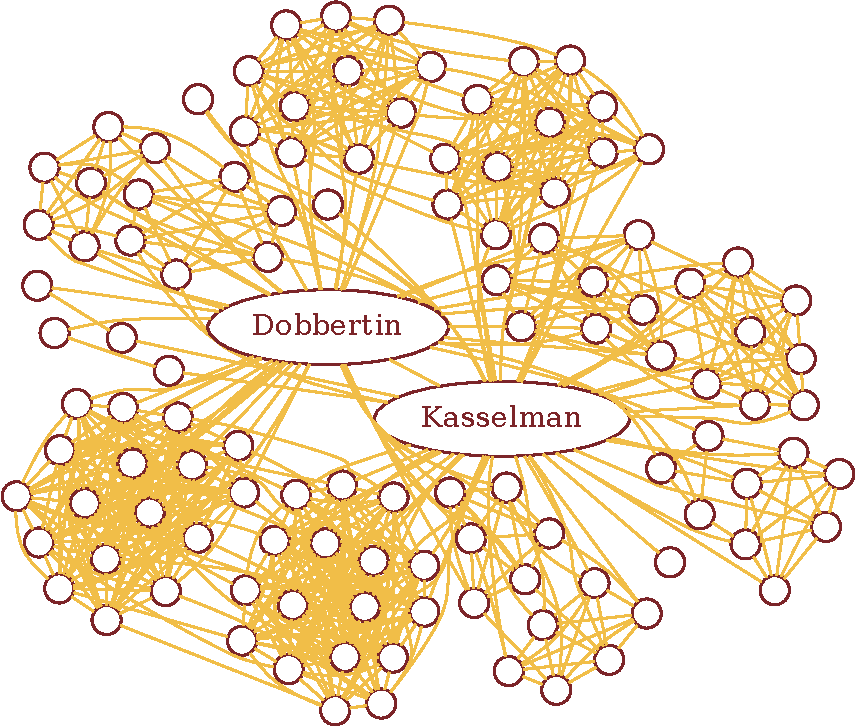
\includegraphics[width=0.5\textwidth]{Figs/graph-intro-crop.pdf}
\caption{A visualization of the heuristic unit-distance neighborhood
  of valid collisions from the Dobbertin and Kasselman collisions.}
\label{Fig:Graph-Intro}
\end{center}
\end{figure}

From a cryptographic perspective, the existence of a feasible collision attack
breaks the requisite properties, thus deprecating the function's use
for trustworthy applications. In many practical instances, however,
communities continue to use deprecated hash functions in a widespread fashion.
One such example of widespread use post-deprecation is the continued use by Git of SHA-1, despite
M. Stevens et al. publishing a full SHA-1 collision in February of 2017
\cite{cryptoeprint:2017:190}. This attack had a bound of $2^{63.1}$
--- faster than the theoretical $2^{80}$ but still requiring significant compute
resources to find.

We seek to address the problem of evaluating the use cases for a collision,
to determine whether or not a collision affects a particular system.
The central thesis of this research is that logical cryptanalysis
allows us to formalize the structure inherent to the underlying hash
function such that new collisions can be found within reasonable time
on commodity hardware.  We assert that when such structure exists, it
is \textbf{imperitive to discontinue use of such hash functions as
  they are fundamentally untrustworthy for critical applications.}  An
example of such structure showing the unit distance neighborhood
(defined in Section \ref{Sec:Terminology}) of the known collisions
from Dobbertin and Kasselman is presented in Figure \ref{Fig:Graph-Intro}.
This paper contributes several techniques to logical cryptanalysis and uses these
techniques to derive metrics of the trustworthiness for hash functions. We claim
the following results are novel in the field:
\begin{itemize}
    \item We define the neighborhood of a class of collisions and show that
        it is frequently non-empty.
    \item We discuss techniques for finding useful collisions within a
        class of collisions using logical cryptanalysis.
    \item We propose additional techniques for building new classes of
        collisions and show that collisions in MD4 can be found inductively.
    \item We propose five universal metrics for evaluating the utility of
        a class of collisions.
\end{itemize}
We propose that collision classes of high utility are closer to a second
preimage attack in the amount of flexibility they provide to an attacker,
whereas classes of low utility may not affect all systems which use a
particular hash function.

The remainder of this paper is organized as follows. In Section
\ref{Sec:Related} we discuss previous results and show how our research
expands upon prior work. In Section \ref{Sec:Terminology}, we discuss the
terminology and notations we use throughout the remainder of the paper.
In Section \ref{Sec:Intuition}, we give the intuition behind measuring
the utility of a collision and motivate why it is useful. In Section
\ref{Sec:Logical}, we present new techniques in logical cryptanalysis to
analyze collisions in hash functions. In Section \ref{Sec:Empirical}, we
discuss the utility of existing collisions under the metrics described in
\ref{Sec:Intuition}. In Section \ref{Sec:Collision}, we discuss new
differential paths and the effectiveness of various techniques presented
in Section \ref{Sec:Logical}. Lastly, in Section \ref{Sec:Impacts}, we
discuss broader impacts of this research.






\section{Related Work} \label{Sec:Related}

This paper draws heavily upon the public cryptanalysis of MD4, the wide
availability of high quality SAT solvers, and previous work in logical
cryptanalysis. In particular, we look at ways that SAT solving can aid
cryptanalysis instead of using cryptanalysis to benchmark SAT solvers. We
then apply them to aid the understanding of attacks against real world
systems, and propose general metrics that target different types of systems.
Towards this, we look at prior work in two main areas: differential and logical
cryptanalysis.

\subsection{On Differential Cryptanalysis}

Differential cryptanalysis has been the major technique behind the discovery
of collisions in cryptographic hash functions. Its importance can be seen
everywhere from X. Wang's attacks on MD4 \cite{Wang2005} to more recent
cryptanalysis of general purpose hash functions such as Murmur3 by
J. Aumasson, D. Bernstein, and M. Bo{\ss}let \cite{murmur3DC}. However, while
differential cryptanalysis plays an important role, techniques for automated
analysis of hash functions are still an emerging area. Further, techniques
are being developed to make hash functions impervious to differential
analysis.

Our work removes the need for finding message modification techniques by
specifying the differential path as part of the SAT formula and letting the
solver find a pair of satisfying messages which follow the differential path
and produce a collision. Further constraints can then be placed upon this
model, such as a chosen prefix or desired start state. We believe performing
these attacks by hand to be difficult, and note that developed message
modification techniques may affect chosen prefixes. Thus, we seek to develop
techniques to replace differential cryptanalysis with logical cryptanalysis.


\subsection{On Logical Cryptanalysis}

Logical cryptanalysis and its encoding as SAT likely started under the work of
F. Massacci in 1999 with his paper titled ``Using walk-SAT and rel-sat for
cryptographic key search''. \cite{Massacci:1999:UWR:1624218.1624261}. However,
much of the early work by F. Massacci was focused on symmetric and asymmetric
ciphers
\cite{Massacci:1999:UWR:1624218.1624261, MASSACCI2000LogicalCA, FIORINI2003101}.
It wasn't until the work of D. Jovanovi{\'{c}} and P. Jani{\v{c}}i{\'{c}}
that exploring collisions in the context of SAT was introduced
\cite{LogicalAnalysis}, and until the work of I. Mironov and L. Zhang that
this was studied for an existing collision class \cite{Mironov2006}.

However, much of the work in this area is focused on benchmarking SAT solvers,
and not on evaluating techniques for using SAT solvers to aid reasoning and
understanding. E. Homsirikamol et al.\ show that SAT solvers can be used to
brute force finding collisions in SHA-3, but with limited utility and limited
to a small number of rounds \cite{Homsirikamol2012}. On the other hand,
advances by V. Nossum in his master's thesis shows that additional work on
encoding is also important: a new 32-bit modular addition circuit produced
shorter run times \cite{nossum_2012}.

We make use of the \textit{bc2cnf} utility by T. Junttila as the basis for
our models \cite{circuits}. This allows us to encode hash functions as generic
structures in the circuit description language and ease the algorithmic
creation of models which build on top of them. We then use CryptoMiniSat5 by
M. Soos to run the models and check for a satisfying witness, often an
example collision \cite{Soos:2009:ESS:1575471.1575502, CryptoMiniSat5}. We
deviate from evaluating the performance of SAT solvers or encodings of models
by instead focusing on evaluating the properties of the hash function. We have
developed new techniques for using a SAT solver to inductively build full
collisions in MD4 from collisions in reduced-round MD4 and to build additional
examples of collision classes from a single instance of a collision in MD4.


\subsection{On Trustworthy Computing}

\textbf{TODO - Assigned @erozier}






\section{Terminology \& Notation}  \label{Sec:Terminology}

\subsection{Conventions}
\begin{itemize}
    \item We assume ordered tuples and strings are indexable via square
        brackets. Occasionally we use subscripts for referring to
        elements of tuples with named members.
    \item We use MD4 as specified in RFC 1320 \cite{rfc1320}.
\end{itemize}

\textbf{TODO}

\subsection{Collisions in Hash Functions}

We use the following terminology when discussing the notion of collisions in
a hash function.

\begin{itemize}
    \item A \textit{cryptographic hash function} is a function:
        \begin{align*}
            h: S_{i} \times B \rightarrow S_{o}
        \end{align*}
        which satisfies the usual properties of cryptographic hash functions
        (preimage, second preimage, collision, deterministic, etc.). We denote
        the input state space as $S_{i}$, the input block space as $B$, and the
        output state space as $S_{o}$. Usually the input state space and the
        output state space are the same, so we omit the subscripts, $S$. We
        assume that these are sets of binary strings of a fixed length. In the
        case of MD4, $S$ is all binary strings of length 128, and $B$ is all
        binary strings of length 512.

    \item An \textit{input} to a hash function is an ordered pair, $i = (s, b)$,
        where $s \in S$ and $b \in B$. The \textit{input space} is simply
        the domain of the hash function, which we denote as $\mathcal{I}$.
        If $i \in \mathcal{I}$ is an input, we reference the state as $i_s$
        and the input block as $i_b$.

    \item We use the term \textit{intermediate state variables} to refer to
        intermediate steps in the computation of a hash function under
        a specific input. Typically these are the outputs of
        one-way compression functions as part of the Merkel-Damg{\aa}rd
        construct. If $i$ is an input to a hash function, we use $I(i)$ to
        denote the intermediate state variables. Formally, this is represented
        as an ordered tuple of binary strings of the size of the updated state.
        In the case of MD4, this is an ordered tuple of cardinality 48, where
        each index is a binary string of length 32, for a total of 1536
        intermediate state variables. We denote the space that $I(i)$ maps
        into as $\mathcal{V}$. We define the number of rounds as $R$.

    \item We use the notation $R(I)$

    \item A \textit{collision}, $L \subseteq \mathcal{I}$ is a subset of the
        input space of a hash function with $\big|L\big| \geq 2$, such that
        there exists an output $v \in S$ such that for all inputs $i \in L$,
        $h(i) = c$.

        \begin{itemize}
            \item We define a \textit{simple collision} to be any collision
                with cardinality exactly two.

            \item We define a \textit{strong collision} to be a collision which
                has multiple blocks which hash to the same output under the same
                input  state. That is, if $L$ is a collision, then
                $\forall i \in L$, $i_s = c$ for some $c \in S$ for $L$ to be
                a strong collision.

            \item We define a \textit{multicollision} to be a collision which
                has multiple input states which hash to the same output under
                a single input block. That is, if $L$ is a collision, then
                $\forall i \in L$, $i_b = c$ for some $c \ in B$ for $L$ to be
                a multicollision.
        \end{itemize}

    \item For a simple collision, we say that the \textit{differential path}
        is the difference between the two sets of intermediate state
        variables. \textbf{TODO -- HELP define formal notation?}
            \begin{itemize}
                \item Signed - Wang's, we don't use.
                \item Unsigned - more common, actually used by us.
            \end{itemize}


    \item A \textit{collision class}, $C$, is an arbitrary differential path.
        If there exists at least one collision pair which has that differential
        path, we call that collision class non-empty. We denote the set of all
        non-empty collision classes as $\mathcal{C}$. When we wish to convert
        between a collision, $c \in L$ and a collision class,
        $C \in \mathcal{C}$, we use the notation $C = \mathcal{C}(c)$.

    \item A \textit{family of collision classes}, $F$, is the indices of a
        collision class, $C$, which have any non-zero difference. That is,
        $F = \{ 0 \leq i \leq R : C[i] \neq 0 \}$.
\end{itemize}

\subsection{Known Collision Classes}

We define the following set of known collision classes.

\begin{itemize}
    \item $C_{Wang}$, to be the collision class introduced by X. Wang
        et al. in \cite{Wang2005}.
    \item $C_{Sasaki}$, to be the collision class introduced by Y. Sasaki
        et al. in \cite{Sasaki2007}.
    \item $C_{Dobbertin}$, to be the collision class introduced by
        H. Dobbertin in \cite{Dobbertin1998}.
    \item $C_{Kasselman}$, to be the collision class introduced by
        P. Kasselman in \cite{KasselmanMD4}.
    \item $C_{Schlaffer}$, to be the collision class introduced by
        M. Schl{\"a}ffer in \cite{Schlaffer2006}.
\end{itemize}

\subsection{Distance Metrics} \label{terminology:distance}

We introduce a distance function, $\delta$, between collision classes by the
number of differences in intermediate rounds deltas. That is, given two
collision classes, $C_1, C_2 \in \mathcal{C}$:
\begin{align}
    \delta(C_1, C_2) = \big| \{ i : C_1[i] \neq C_2[i] \} \big|
\end{align}
We extend this distance function to include an \textit{absolute} distance,
measuring the number of intermediate rounds with non-zero differences.
We notate this as $\delta(C_1)$.

We can define a similar distance function, $\Delta$, between families of
collision classes by cardinality of the symmetric difference in the two
collision families. That is, given two families of collision classes,
$F_1, F_2 \in \mathcal{F}$:
\begin{align}
    \Delta(F_1, F_2) = \big| (F_1 \cup F_2) \setminus (F_1 \cap F_2) \big|
\end{align}
This is convenient for when the specifics of the differential path do not
matter, merely that there exists at least one collision class of the specified
form.

We introduce this distance function as a heuristic measure of the
sensitivity of the hash function to small changes in the input.

\subsection{Neighborhoods}

We define the neighborhood of a collision class, $C \in \mathcal{C}$, to be the
set of all other non-empty collision classes at a fixed distance,
$d \in \mathbb{N}$, from $C$. That is:
\begin{align}
    N(C, d) & = \{ C_j \in \mathcal{C} : \delta(C, C_j) = d \} \\
    N(C) & = N(C, 1)
\end{align}
For instance, $C_{Wang} \in N(C_{Sasaki}, 21)$. The distance parameter, $d$,
may optionally be omitted, in which case the unit distance is implied. Thus,
$C_{Kasselman} \in N(C_{Dobbertin})$.

We can similarly define the neighborhood of a family of collision classes,
$F \in \mathcal{F}$, to be the set of all other families of collision classes
at a fixed distance, $d \in \mathbb{N}$, from $F$. That is:
\begin{align}
    \mathcal{N}(F, d) & = \{ F_j \in \mathcal{F} : \delta(F, F_j) = d \} \\
    \mathcal{N}(F) & = N(F, 1)
\end{align}
The distance parameter, $d$, may optionally be omitted, in which case the unit
distance is implied.

Neighborhoods can be classified into three types: \textit{expansion},
\textit{internal}, and \textit{mixed}. Let $d$ be fixed. An \textit{expansion}
neighborhood of a collision class, $C \in \mathcal{C}$, is the neighborhood
restricted only to those collision classes which only differ in rounds external
to the collision family of $C$. An \textit{internal} neighborhood of $C$ is the
neighborhood restricted only to those collision classes which differ in rounds
internal to the collision family of $C$. A \textit{mixed} neighborhood of $C$
is the neighborhood restricted only to collisions which differ in a round
internal and a round external to the collision family of $C$. That is:
\begin{align*}
    N_{exp}(C, d) = \{ & C_{j} \in N(C, d) : \forall i \in F(C), C_j[i] = C[i] \} \\
    N_{int}(C, d) = \{ & C_{j} \in N(C, d) : \forall i \not\in F(C), C_j[i] = C[i] \} \\
    N_{mix}(C, d) = \{ & C_{j} \in N(C, d) : \exists i \in F(C), C_j[i] \neq C[i] \\
        & \text{ and } \exists k \not\in F(C), C_j[k] \neq C[k] \}
\end{align*}

When the neighborhood defined by $\delta = 1$ is frequently non-empty
we assert that sufficient structure exists in the underlying hash
function such that logical cryptanalysis via 3-CNF-SAT becomes
feasible.  This condition is thus sufficient to render the underlying
hash function \textbf{untrustworthy}.  Conversely it is a necessary
condition (but possibly insufficient) that a trustworthy hash function
has an empty neighborhood defined by $\delta = 1$.

Furthermore this condition extends to $\delta = d$ for some small
value of $d$ as determined by computational resources such that $d$
becomes a trustworthiness metric under constraints of current
3-CNF-SAT solving capabilities within reasonable time bounds.

\section{Intuition on the Utility of a Collision} \label{Sec:Intuition}

\textbf{TODO - audit introductory paragraphs}

We seek to build new intuition about collisions in hash functions
and particularly collisions in MD4. By developing techniques using logical
cryptanalysis, we seek to complement and extend the results from
differential cryptanalysis. In particular, we wish to use logical cryptanalysis
to discuss the impacts of collisions in real-world systems. In this paper,
we introduce and give justification for general techniques, and present some
results of these techniques.

To begin, real world systems are most vulnerable to two attacks: the preimage
and second preimage. For systems relying on password validation via
comparing two hashes, preimage attacks would allow inverting the hash,
increasing the risk associated with losing a database of hashed passwords.
On the other hand, systems relying on message validation, such as signature
checks or file integrity checks would be easily broken with fast second
preimage techniques. Both of these attacks are intractable, thus protecting
real-world systems. However, much research has been devoted to collision
attacks, producing efficient results.

Thus, we seek to evaluate the relative difference between a collision
attack and second preimage attacks, to give some measure of distance between
them. Several high profile attacks against hash function usage have been
made. For MD5, these include cloning a CA certificate \cite{Stevens2009}
and creating malicious executables \cite{MD5Executables}. For SHA-1, a pair of
PDFs with the same hash \cite{cryptoeprint:2017:190}. However, many of these
techniques exploit not the hash, but the flexibility of the file format,
relying instead on embedding arbitrary, collidable data and later checking for
the presence of one of the matching blocks. This is especially obvious in the
MD5 executable and SHA-1 PDF attacks. The work by M. Stevens to perform the
CA Collision, on the other hand, was a chosen prefix attack extending
previous work from 2007 \cite{Stevens2007}.

Seeing the need to evaluate how much flexibility exists in a collision,
we propose the following metrics for evaluating the utility of a collision
class:
\begin{enumerate}
    \item The number of unique differentials a collision class has.
    \item The number of unit-step neighbors a collision class has.
    \item The maximum count of zeros in a the binary representation of a
        colliding block (and likewise with ones).
    \item Whether there exists a block which collides under multiple initial
        values.
    \item Whether or not zero, one, or both of the blocks in a collision may
        be of ASCII values under any input block difference.
\end{enumerate}
Note that the first three are quantitative measures providing some measure of
flexibility of a collision class, whereas the latter two are merely looking
for a single witness having such a property. Depending on the scenario,
specific properties of a collision may be of more interest than others.

The first metric evaluates the flexibility of the differential path. A
differential path with more flexibility will have more differentials which
produce blocks with the given differential path. More differentials implies
a greater flexibility in choice of colliding block, and possibly allows
for multiple collisions for a given colliding block. Furthermore, a collision
with more differentials is more likely to satisfy the last metric, having a
pair of blocks--both ASCII--which produce a collision.

The second metric evaluates the density of the neighborhood of a collision
class. If a collision resides in a dense neighborhood, it provides more
possible collision classes to search for a second preimage, chosen prefix, or
other structure desired in a collision. If, however, a collision class has no
neighbors, then it cannot be used to find other possible classes for other
input blocks.

The maximum quantity of zeros (or ones) in the binary representation of a
block serve as a measure of the extremes to which a collision can be pushed.
This can additionally be extended to any suitable bit pattern in any base to
provide a more relevant metric as desired by the system under study.

The fourth metric evaluates the utility of a collision when the internal state
of the hash function is unknown. If a collision occurs under multiple initial
values, this could be used to attack some systems where user provided input is
appended to unknown data and then hashed. If a block collides under a suitably
large number of initial values, the attack becomes highly likely to occur
successfully. However, measuring the exact number of initial values a block
collides under is beyond the scope of this work.

The last metric is similar to the third in that it looks for specific bit
patterns in a collision. ASCII is one example of a widely used constraint
system. Further examples, such as JSON, XML, etc., may likewise be
supplemented based on the specifics of the system.

If a collision class satisfies many of these properties, then it is more
flexible and thus more likely to be used to target deployed systems. If,
however, a collision class does not satisfy these properties, its impact is
likely severely limited in scope, and may not provide useful information to
find other collision classes which have higher utility.








\section{Techniques for Logical Cryptanalysis} \label{Sec:Logical}

\begin{figure*}
\begin{center}
  \begin{subfigure}{\textwidth}
    
\includegraphics[width=\textwidth]{Figs/differential-1289.png}
    \caption{Collision 1289}
    \label{Fig:1289}
  \end{subfigure}\\
  \begin{subfigure}{\textwidth}
    
\includegraphics[width=\textwidth]{Figs/differential-1250.png}
    \caption{Collision 1250}
    \label{Fig:1250}
  \end{subfigure}\\
  \begin{subfigure}{\textwidth}
    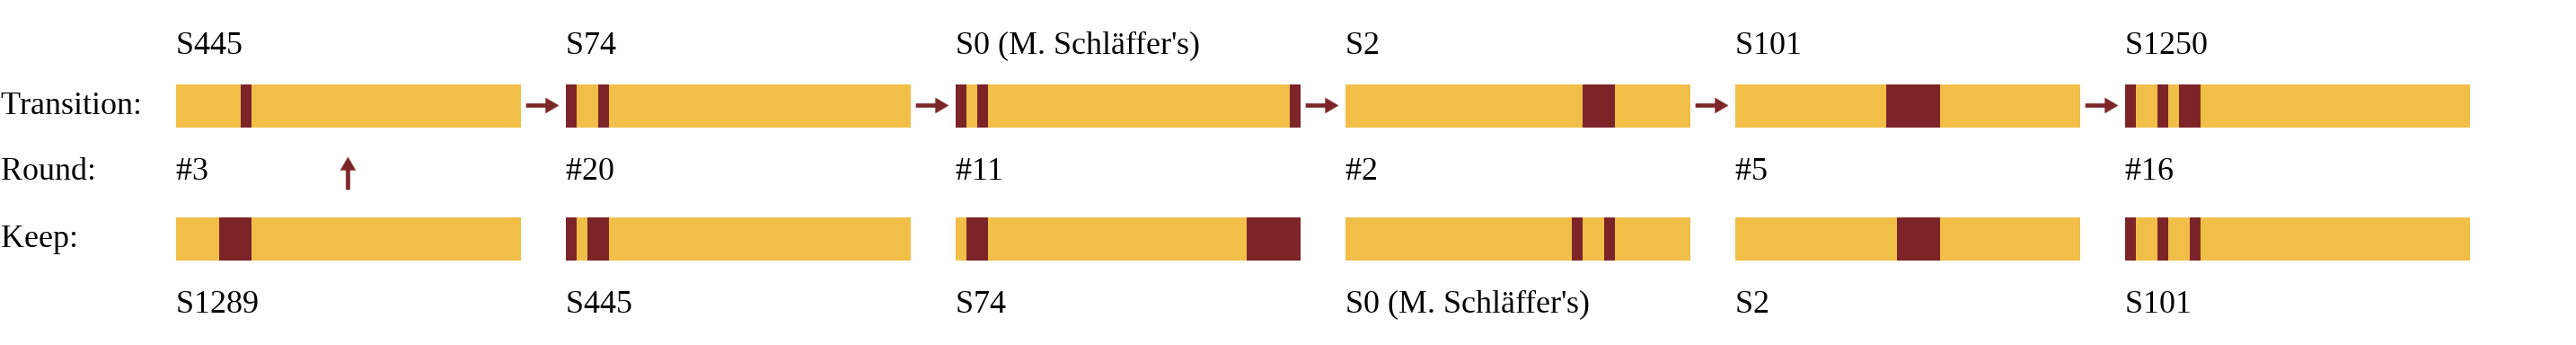
\includegraphics[width=\textwidth]{Figs/transitions.png}
    \caption{Differential Path Transitions}
    \label{Fig:Transitions}
  \end{subfigure}\\
\end{center}
\end{figure*}

The following techniques have been extensively tested on MD4 and partially
tested on MD5 and are believed to apply fully to MD5. They likely apply to any
hash function with similar structure, but as of yet, are untested.


\subsection{Distance Metrics}

We find justification for the distance metric defined in Section
\ref{terminology:distance} in the existing literature on MD4:
H. Dobbertin's \cite{Dobbertin1998} and P. Kasselman's \cite{KasselmanMD4}
collision classes have distance $\delta(C_{Dobbertin}, C_{Kasselman}) = 1$
under this metric. The distance function allows us to find collision classes
based off of existing classes. By limiting ourselves to unit distances, we
maximally reuse an existing collision and limit the amount of work the SAT
solver needs to do. Further, rather than searching for any unit-distance
new collision classes, we can easily split our search to look in each of the
48 rounds of MD4, allowing us to parallelize the search for neighbors.

Refer to Table \ref{table:distance} for the distances between existing
collisions in MD4.

\begin{table}
    \caption{Distance between Existing Collision Classes}
    \label{table:distance}
    \begin{tabular}{c c c c c c c}
        & X. W. & Y. S. & P. K. & H. D. & M. S. & Absolute \\
        X. Wang's & 0 & 21 & 26 & 27 & 12 & 18 \\
        Y. Sasaki's & & 0 & 25 & 26 & 2 & 16 \\
        P. Kasselman's &  &  & 0 & 1 & 25 & 11 \\
        H. Dobbertin's &  &  &  & 0 & 26 & 12 \\
        M. Schl{\"a}ffer's &  &  &  &  & 0 & 17 \\
    \end{tabular}
\end{table}

We find justification for the distance metric $\Delta$ in the existing
literature due to collisions by  X. Wang \cite{cryptoeprint:2004:199} and
M. Schl{\"a}ffer \cite{Schlaffer2006}. Their respective families are:

\begin{align*}
F(C_{Wang}) &=& (1, 2, 3, 5, 6, 7, 8, 9, 10, 11, 12, \textbf{13}, 15, 16, 19, 20, 35, 36)\\
F(C_{Schlaffer}) &=& (1, 2, 3, 5, 6, 7, 8, 9, 10, 11, 12, 15, 16, 19, 20, 35, 36)
\end{align*}

\subsection{Family Similarity}

We define a relation among families of collisions across rounds as follows.
Let $F_1$ and $F_2$ be two different families of collisions. Then we say that
$F_1$ and $F_2$ are \textit{similar}, and notate it $F_1 \precsim F_2$, if
$R(F_1) \leq R(F_2)$ and $F_1 \subseteq F_2$. Note that, when
$R(F_1) = R(F_2)$, this is equivalent to saying that $F_2$ is in some
expansion neighborhood of $F_1$. Further, when $R(F_1) < R(F_2)$ and
$F_1 = F_2$, then we say that $F_2$ is the \textit{trivial extension} of
$F_1$.

We claim that the following statements are true for MD4:
\begin{enumerate}
    \item For every $F \in \mathcal{F}$, there exists $F'$ such that
        $F' \precsim F$ and $R(F') + 4 = R(F)$.
    \item For every $F \in \mathcal{F}$, there exists $F'$ such that
        $F \precsim F'$.
\end{enumerate}

From an intuitive standpoint, what this says is that collisions have
witnesses for their existence in reduced round versions of the function, and
further, that it is sufficient to search reduced round versions to find
candidates for extension into additional rounds. This likely derives from
the iterative construction of MD4 and the particular choice of block schedule.

\textbf{TODO -- Empirical justification / graphical representation?}


\subsubsection{Collision Class Similarity}

We claim that the aforementioned statements hold when considering individual
collision classes instead of families of collision classes, but with less
likelihood. That is, we can transplant an $n$ round collision into an $n+4$
round and consider a neighborhood around it to find a new collision.

\subsubsection{Second Preimage Similarity}

If the models are constrained for a second preimage, we note that attack again
works, but requires searching wider and wider differential paths in small round
sizes. In particular, despite strong evidence for this pattern holding in
$n \leq 24$ rounds, outside of the collision family $\{0, 16\}$ in both 28 and
32 round MD4--which does not extend any further--we have been unable to find
any other differential path in those rounds by exhaustive brute force search
up to a differential path of length 8. Further searches have been done of
36, 40, 44, and 48 rounds up to a differential path of length 5 with a similar
lack of results. Thus we believe the general technique to hold, but the size
of the search space for a second preimage becomes prohibitively large, and
further, that differential paths become sufficiently long to prohibit easy
finding of second preimages.

\subsubsection{Chosen Prefix Similarity}

Unlike second preimage attacks, chosen prefix attacks have a higher likelihood
of working, and give better results. However, we have found that most chosen
prefixes work in the neighborhoods of existing collisions, and thus are not
convinced that inductively building a chosen prefix collision is a useful
technique by itself.


\subsection{Unjustified Performance Observations}

We share the general tips for working with models of MD4 from a SAT solver
performance perspective, without justification for results. Note that these
results may be limited in usefulness and may not be uniformly applicable.
\begin{itemize}
    \item Unless searching for a second preimage or chosen prefix with
        sufficient number of bits ($\geq 128$), we find models perform better
        leaving the initial state unconstrained.
    \item Adding ASCII block constraints significantly and negatively impact
        the performance of finding a collision.
    \item Keeping a small search radius on neighborhoods involving families
        of collision classes is important for good performance. However,
        once sufficient witnesses have been found across rounds, missing
        families within the round can be found by various filling-in
        techniques through applying the $\precsim$ relation.
\end{itemize}






\section{Empirical Results:\\The Utility of Existing Collisions}
\label{Sec:Empirical}

\textbf{TODO -- Introduction?}

\subsection{Unique Differentials}

Table \ref{table:differentials} states the number of unique differentials,
including the specified one, which produces a differential path conforming to
each of the collision classes. We note in particular that while Y. Sasaki's
attack is generally an improvement upon X. Wang's, Y. Sasaki's attack has fewer
input block differentials and thus less flexibility in this aspect. Further,
M. Schl{\"a}ffer's attack -- also building off the work of X. Wang -- has the
same number of differentials and is thus also more flexible than Y. Sasaki's.

\begin{table}
    \caption{Number of Differentials for Existing Collision Classes}
    \label{table:differentials}
    \begin{tabular}{c c c c}
        \textbf{Attack} & \textbf{Size} & \textbf{Attack} & \textbf{Size} \\
        X. Wang's & 64 & Y. Sasaki's & 4 \\
        H. Dobbertin's & 32 & P. Kasselman's & 32 \\
        M. Schl{\"a}ffer's & 64 & & \\
    \end{tabular}
\end{table}

\subsection{Unit-Step Neighborhood} \label{empirical:neighborhood}

\begin{figure}
\begin{center}
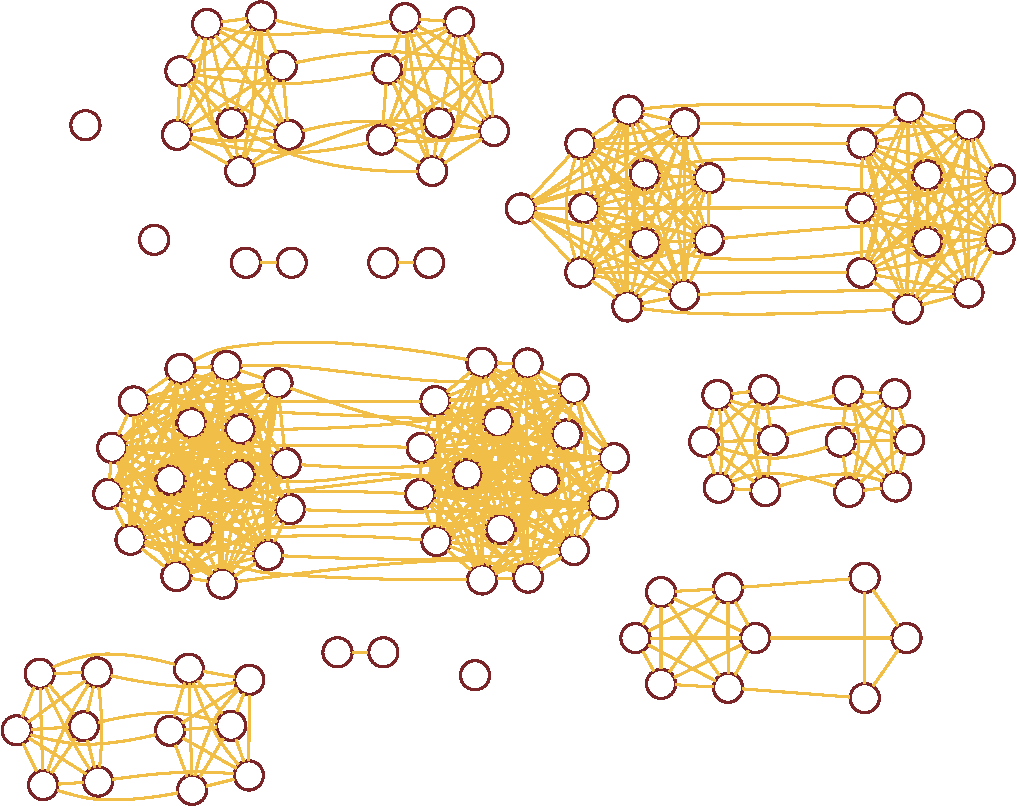
\includegraphics[width=0.5\textwidth]{Figs/graph-clique-crop.pdf}
\caption{}
\label{Fig:Graph-Clique}
\end{center}
\end{figure}

\begin{figure}
\begin{center}
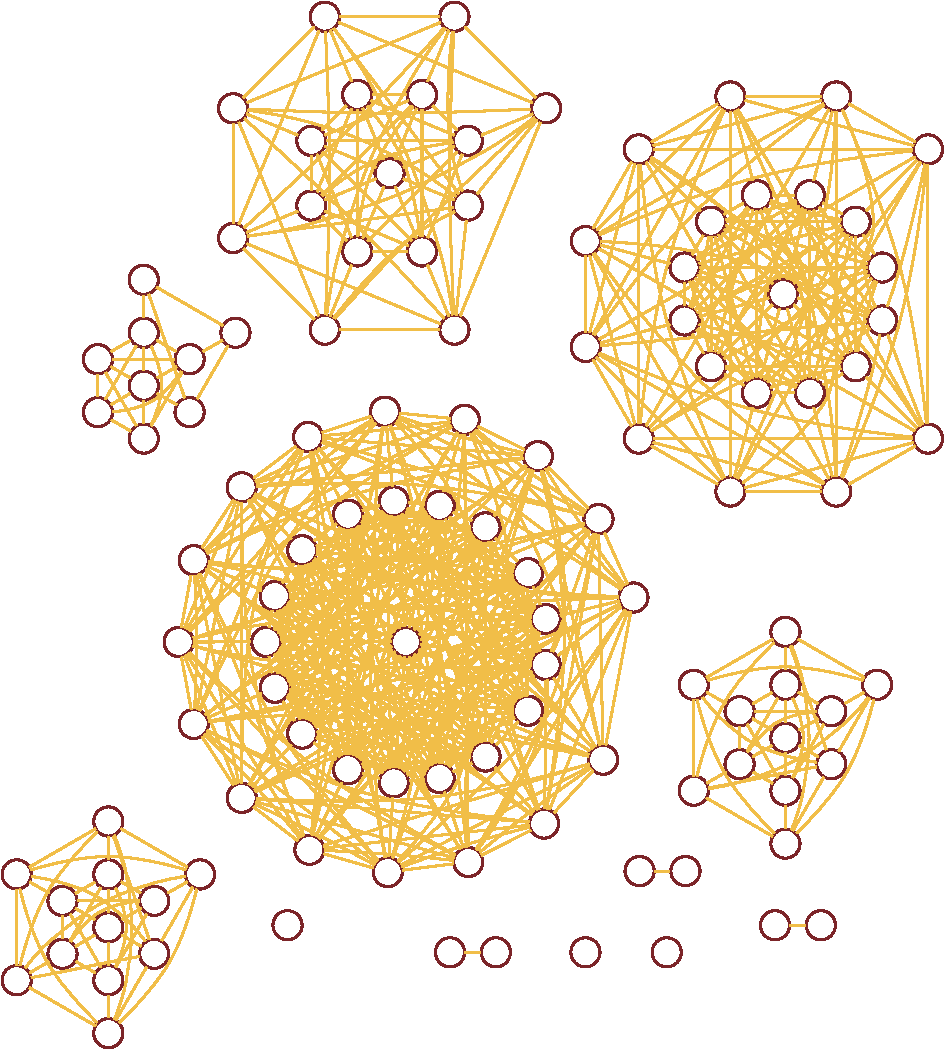
\includegraphics[width=0.5\textwidth]{Figs/graph-neighborhood-crop.pdf}
\caption{}
\label{Fig:Graph-Neighborhood}
\end{center}
\end{figure}

Refer to Table \ref{table:neighborhood} for the sizes of neighborhoods
of existing collisions. In particular, note that both Y. Sasaki's attack and
M. Schl{\"a}ffer's attack -- which both claimed to improve upon X. Wang's
attack--have larger neighborhood sizes, and likewise with P. Kasselman's
attack which improved upon H. Dobbertin's attack. Thus, the newer collisions
occur in more dense subsets of the collision class space.

\begin{table}
    \caption{Neighborhood Sizes for Existing Collision Classes}
    \label{table:neighborhood}
    \begin{tabular}{c c c c}
        \textbf{Attack} & \textbf{Size} & \textbf{Attack} & \textbf{Size} \\
        X. Wang's & 54 & Y. Sasaki's & 157 \\
        H. Dobbertin's & 55 & P. Kasselman's & 60 \\
        M. Schl{\"a}ffer's & 100 & & \\
    \end{tabular}
\end{table}


\subsection{Zeroes}

See table \ref{table:zeroes} for the maximum count of zeroes in a block
for existing collisions. Note that X. Wang's attack is the leader, with 509
maximum zero bits in the collision pair. Further, while Y. Sasaki improved
the bound in other areas, this was not one of them. Of note too,
H. Dobbertin's and P. Kasselman's collisions are essentially identical in
this metric.

\begin{table}
    \caption{Number of Zeroes in a Colliding Block}
    \label{table:zeroes}
    \begin{tabular}{c c c c}
        \textbf{Attack} & \textbf{Count} & \textbf{Attack} & \textbf{Count} \\
        X. Wang's & 509 & Y. Sasaki's & 494 \\
        H. Dobbertin's & 504 & P. Kasselman's & 504 \\
        M. Schl{\"a}ffer's & 506 & & \\
    \end{tabular}
\end{table}



\subsection{Multicollisions}

We note that while these collisions are state independent and include
multicollisions, none of these attacks are always multicollisions. Many of the
blocks we've found only collide under the initial state value. Because of this,
these collisions are only useful if you know the current state where a
colliding pair is to be injected. Thus, this is one area in which collisions
could potentially improve.


\subsection{ASCII Blocks}

See Table \ref{table:ascii} for results of finding ASCII block pairs. Note that
this table validates P. Kasselman's and H. Dobbertin's results of finding
two ASCII block messages. However, these results do not hold for later
collisions by X. Wang, Y. Sasaki, or M. Schl{\"a}ffer. Thus, while the latter
attacks have been viewed as being of better quality, under this particular
metric, P. Kasselman's and H. Dobbertin's collision classes are better.

\begin{table}
    \caption{ASCII Blocks in Existing Collision Classes}
    \label{table:ascii}
    \begin{tabular}{c c c}
        \textbf{Attack} & \textbf{Single Block} & \textbf{Both Blocks} \\
        X. Wang's & true & false \\
        Y. Sasaki's & true & false \\
        P. Kasselman's & true & \textbf{true} \\
        H. Dobbertin's & true & \textbf{true} \\
        M. Schl{\"a}ffer's & true & false \\
    \end{tabular}
\end{table}


\subsection{Recapitulation}

Overall, we feel that while the given collision classes have value and utility,
they do not constitute full second preimage attacks. Further, simple
neighborhood searches do not lead to collisions in every case. Therefore,
additional techniques are necessary for expanding the collision neighborhood.




\section{New Collisions} \label{Sec:Collision}

Through the exploration of the neighborhood technique, we have found over
35,000 new differential paths which originated from the five original
collisions in MD4. This shows that the neighborhood definition is sufficient
to produce a large quantity of new collision classes. Further, we give
evidence for propagating neighborhoods across reduced round versions of MD4.

\subsection{Extensions of Prior Work}

We noted in table \ref{table:neighborhood} that the unit-step neighborhood of
the existing attacks were non-empty. By repeatedly expanding neighborhoods of
known collision classes, we can construct paths in the collision space. We
made the following observations:

\begin{enumerate}
    \item The space of collision classes is not smooth under the unit distance
        relation. That is, starting at $C_{Schlaffer}$ and evaluating
        successive neighborhoods, moving towards $C_{Wang}$ whenever the
        distance decreases does not lead to a simple path of length
        $\delta(C_{Schlaffer}, C_{Wang}) = 17$. Our lower bound on the actual
        distance is 29, but after 14 rounds of expansion, we only reduced the
        distance to 15.
    \item Even under successive unit neighborhoods, the family of input block
        differentials remains roughly the same among successive neighborhoods.
        This can be partially counteracted by moving to reduced-round spaces,
        evaluating the neighborhood, and expanding back to a collision in
        full-round MD4. That is, there is a detectable signature of sharing
        significant input block differential structure with the original
        collision. With 35,918 unique classes of collisions which had 176
        unique families of collisions, there were only three unique families
        of input block differentials: those of the starting collision classes.
\end{enumerate}

This last point shows that, while there may be a number of unique differentials
for a given collision class, and potentially many collision classes within
some neighborhood of the original collision class, by analyzing the structure
of the input block differential, systems can potentially prohibit successful
collision attacks by preventing structures of input block differences.

\textbf{TODO - figures and graphics on dataset}



\section{Discussion of Impacts} \label{Sec:Impacts}

\textbf{TODO} - Recap impacts on real-world systems like MD5, SHA-1, etc.

% An example of a floating figure using the graphicx package.
% Note that \label must occur AFTER (or within) \caption.
% For figures, \caption should occur after the \includegraphics.
% Note that IEEEtran v1.7 and later has special internal code that
% is designed to preserve the operation of \label within \caption
% even when the captionsoff option is in effect. However, because
% of issues like this, it may be the safest practice to put all your
% \label just after \caption rather than within \caption{}.
%
% Reminder: the "draftcls" or "draftclsnofoot", not "draft", class
% option should be used if it is desired that the figures are to be
% displayed while in draft mode.
%
%\begin{figure}[!t]
%\centering
%\includegraphics[width=2.5in]{myfigure}
% where an .eps filename suffix will be assumed under latex,
% and a .pdf suffix will be assumed for pdflatex; or what has been declared
% via \DeclareGraphicsExtensions.
%\caption{Simulation results for the network.}
%\label{fig_sim}
%\end{figure}

% Note that the IEEE typically puts floats only at the top, even when this
% results in a large percentage of a column being occupied by floats.


% An example of a double column floating figure using two subfigures.
% (The subfig.sty package must be loaded for this to work.)
% The subfigure \label commands are set within each subfloat command,
% and the \label for the overall figure must come after \caption.
% \hfil is used as a separator to get equal spacing.
% Watch out that the combined width of all the subfigures on a
% line do not exceed the text width or a line break will occur.
%
%\begin{figure*}[!t]
%\centering
%\subfloat[Case I]{\includegraphics[width=2.5in]{box}%
%\label{fig_first_case}}
%\hfil
%\subfloat[Case II]{\includegraphics[width=2.5in]{box}%
%\label{fig_second_case}}
%\caption{Simulation results for the network.}
%\label{fig_sim}
%\end{figure*}
%
% Note that often IEEE papers with subfigures do not employ subfigure
% captions (using the optional argument to \subfloat[]), but instead will
% reference/describe all of them (a), (b), etc., within the main caption.
% Be aware that for subfig.sty to generate the (a), (b), etc., subfigure
% labels, the optional argument to \subfloat must be present. If a
% subcaption is not desired, just leave its contents blank,
% e.g., \subfloat[].


% An example of a floating table. Note that, for IEEE style tables, the
% \caption command should come BEFORE the table and, given that table
% captions serve much like titles, are usually capitalized except for words
% such as a, an, and, as, at, but, by, for, in, nor, of, on, or, the, to
% and up, which are usually not capitalized unless they are the first or
% last word of the caption. Table text will default to \footnotesize as
% the IEEE normally uses this smaller font for tables.
% The \label must come after \caption as always.
%
%\begin{table}[!t]
%% increase table row spacing, adjust to taste
%\renewcommand{\arraystretch}{1.3}
% if using array.sty, it might be a good idea to tweak the value of
% \extrarowheight as needed to properly center the text within the cells
%\caption{An Example of a Table}
%\label{table_example}
%\centering
%% Some packages, such as MDW tools, offer better commands for making tables
%% than the plain LaTeX2e tabular which is used here.
%\begin{tabular}{|c||c|}
%\hline
%One & Two\\
%\hline
%Three & Four\\
%\hline
%\end{tabular}
%\end{table}


% Note that the IEEE does not put floats in the very first column
% - or typically anywhere on the first page for that matter. Also,
% in-text middle ("here") positioning is typically not used, but it
% is allowed and encouraged for Computer Society conferences (but
% not Computer Society journals). Most IEEE journals/conferences use
% top floats exclusively.
% Note that, LaTeX2e, unlike IEEE journals/conferences, places
% footnotes above bottom floats. This can be corrected via the
% \fnbelowfloat command of the stfloats package.




\section{Conclusion} \label{Sec:Conclusion}
The conclusion goes here.



\section{Future Work}

The framework can be seen here \textbf{TODO}. Complete data set available
upon request.



% conference papers do not normally have an appendix


% use section* for acknowledgment
\section*{Acknowledgments}

The authors would like to thank the Department of Electrical and Computer
Engineering and XXXXX XXXXX for providing hardware.





% trigger a \newpage just before the given reference
% number - used to balance the columns on the last page
% adjust value as needed - may need to be readjusted if
% the document is modified later
%\IEEEtriggeratref{8}
% The "triggered" command can be changed if desired:
%\IEEEtriggercmd{\enlargethispage{-5in}}

% references section

% can use a bibliography generated by BibTeX as a .bbl file
% BibTeX documentation can be easily obtained at:
% http://mirror.ctan.org/biblio/bibtex/contrib/doc/
% The IEEEtran BibTeX style support page is at:
% http://www.michaelshell.org/tex/ieeetran/bibtex/
\bibliographystyle{IEEEtran}

% argument is your BibTeX string definitions and bibliography database(s)
\bibliography{thesis}




% that's all folks
\end{document}
